\documentclass{article}
\usepackage{amsmath, sfmath, multicol, tkz-euclide, array, enumerate, tcolorbox, tabularray}
\renewcommand{\familydefault}{\sfdefault}
\setlength{\parindent}{0cm}
\pagestyle{empty}
\usepackage[left=1in, top=0.5in, right=1in, bottom=0.5in]{geometry}
\tikzset{>=stealth}
\tcbset{colback=white}

\newcounter{example}[section]
\newenvironment{example}[1][]{\refstepcounter{example}\par\medskip
   {\color{red}\textbf{Example~\theexample. #1}}}{\medskip}

\begin{document}

\section*{Midsegments of Triangles}

\begin{tcolorbox}[colframe=orange!70!white, coltitle=black, title=\textbf{Today I Can}]
\begin{enumerate}
    \item Use properties of midsegments to solve problems.
\end{enumerate}
\end{tcolorbox}
\smallskip

\begin{tcolorbox}[colframe=black!20!white, opacitybacktitle=0.1, coltitle=black, title=\textbf{Midsegment}]
A segment connecting the midpoints of 2 sides of a triangle.
\end{tcolorbox}

\begin{tcolorbox}[colframe=black!20!white, opacitybacktitle=0.1, coltitle=black, title=\textbf{Triangle Midsegment Theorem}]
The midsegment of a triangle is parallel to to a side and half its length. \newline 

\begin{minipage}{0.55\textwidth}
\begin{itemize}
    \item $\overline{DE} \parallel \overline{AC}$
    \item $DE = \frac{1}{2}AC$
\end{itemize}
\end{minipage}
\begin{minipage}{0.4\textwidth}
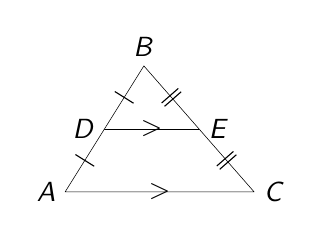
\begin{tikzpicture}[scale=0.8]
\tkzDefPoints{0/0/A, 1.25/2/B, 3/0/C}
\tkzDrawPolygon(A,B,C)
\tkzDefMidPoint(A,B)
\tkzGetPoint{D}
\tkzDefMidPoint(B,C)
\tkzGetPoint{E}
\tkzDrawSegment(D,E)
\tkzLabelPoints[left](A,D)
\tkzLabelPoints[right](C,E)
\tkzLabelPoints[above](B)
\tkzMarkSegments[mark=|](A,D B,D)
\tkzMarkSegments[mark=||](B,E C,E)
\tkzDefMidPoint(A,C)
\tkzGetPoint{F}
\node at (F) {$>$};
\tkzDefMidPoint(D,E)
\tkzGetPoint{G}
\node at (G) {$>$};
\end{tikzpicture}
\end{minipage}
\end{tcolorbox}

\begin{example}
Find each length.
\begin{multicols}{2}
\begin{enumerate}[(a)]
    \item $BD$
    \item $ED$
\end{enumerate}
\end{multicols}
\begin{minipage}{0.5\textwidth}
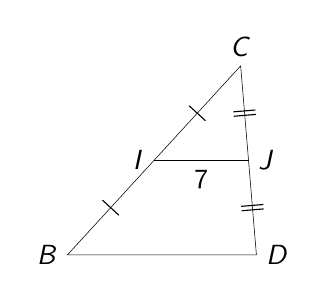
\begin{tikzpicture}[scale=0.8]
\tkzDefPoints{0/0/B, 3/0/D, 2.75/3/C}
\tkzDrawPolygon(B,D,C)
\tkzDefMidPoint(B,C)
\tkzGetPoint{I}
\tkzDefMidPoint(C,D)
\tkzGetPoint{J}
\tkzDrawSegment(I,J)
\tkzLabelPoints[left](B,I)
\tkzLabelPoints[above](C)
\tkzLabelPoints[right](J,D)
\tkzLabelSegment[below](I,J){7}
\tkzMarkSegments[mark=|](B,I I,C)
\tkzMarkSegments[mark=||](C,J D,J)
\end{tikzpicture}
\end{minipage}
\begin{minipage}{0.4\textwidth}
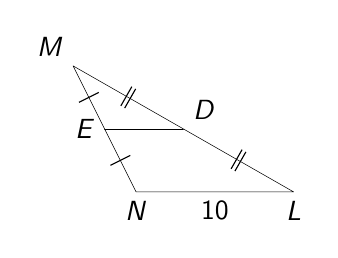
\begin{tikzpicture}[scale=0.8]
\tkzDefPoints{0/0/N, 2.5/0/L, -1/2/M}
\tkzDrawPolygon(N,L,M)
\tkzLabelPoints[below](N,L)
\tkzLabelPoints[above left](M)
\tkzLabelSegment[below](N,L){10}
\tkzDefMidPoint(M,N)
\tkzGetPoint{E}
\tkzDefMidPoint(M,L)
\tkzGetPoint{D}
\tkzDrawSegment(E,D)
\tkzLabelPoints[left](E)
\tkzLabelPoints[above right](D)
\tkzMarkSegments[mark=|](M,E N,E)
\tkzMarkSegments[mark=||](M,D L,D)
\end{tikzpicture}
\end{minipage}
\end{example}

\vspace{0.25in}

\begin{example}
Solve for $x$ in each.
\begin{multicols}{2}
\begin{enumerate}[(a)]
    \item \mbox{} \newline 
    \item \mbox{} \newline 
\end{enumerate}
\end{multicols}
\begin{minipage}{0.5\textwidth}
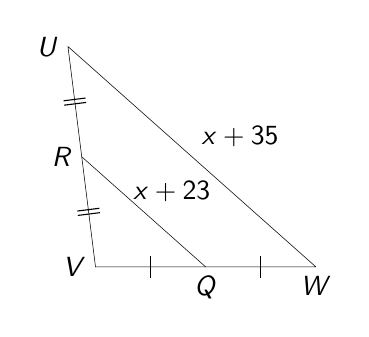
\begin{tikzpicture}[scale=0.7]
\tkzDefPoints{0/0/V, 4/0/W, -0.5/4/U}
\tkzDrawPolygon(U,V,W)
\tkzDefMidPoint(V,W)
\tkzGetPoint{Q}
\tkzDefMidPoint(U,V)
\tkzGetPoint{R}
\tkzDrawSegment(R,Q)
\tkzMarkSegments[mark=|](V,Q Q,W)
\tkzMarkSegments[mark=||](V,R R,U)
\tkzLabelSegment[above right,xshift=-0.1in](R,Q){$x+23$}
\tkzLabelSegment[above right](U,W){$x+35$}
\tkzLabelPoints[left](U,V,R)
\tkzLabelPoints[below](Q,W)
\end{tikzpicture}
\end{minipage}
\begin{minipage}{0.4\textwidth}
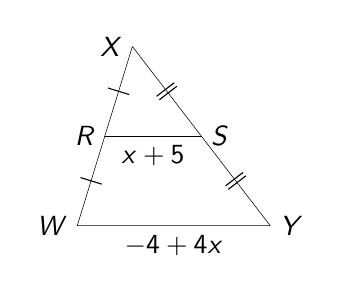
\begin{tikzpicture}[scale=0.7]
\tkzDefPoints{0/0/W, 3.5/0/Y, 1/3.25/X}
\tkzDrawPolygon(W,Y,X)
\tkzDefMidPoint(X,W)
\tkzGetPoint{R}
\tkzLabelPoints[left](X,R,W)
\tkzDefMidPoint(X,Y)
\tkzGetPoint{S}
\tkzLabelPoints[right](S,Y)
\tkzDrawSegment(R,S)
\tkzLabelSegment[below](R,S){$x+5$}
\tkzLabelSegment[below](W,Y){$-4+4x$}
\tkzMarkSegments[mark=|](X,R R,W)
\tkzMarkSegments[mark=||](X,S Y,S)
\end{tikzpicture}
\end{minipage}
\end{example}

\newpage 

\begin{example}
Find $WY$   \newline 

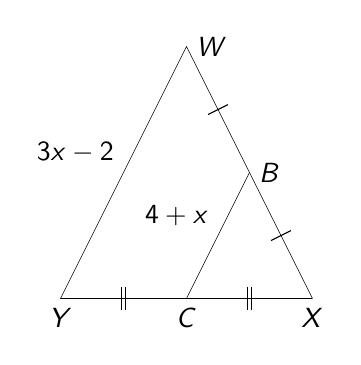
\begin{tikzpicture}[scale=0.8]
\tkzDefPoints{0/0/Y, 4/0/X, 2/4/W}
\tkzDrawPolygon(X,Y,W)
\tkzDefMidPoint(Y,X)
\tkzGetPoint{C}
\tkzDefMidPoint(W,X)
\tkzGetPoint{B}
\tkzDrawSegment(B,C)
\tkzLabelPoints[below](X,C,Y)
\tkzLabelPoints[right](B,W)
\tkzLabelSegment[above left](B,C){$4+x$}
\tkzLabelSegment[above left](W,Y){$3x-2$}
\tkzMarkSegments[mark=|](B,W X,B)
\tkzMarkSegments[mark=||](C,Y C,X)0
\end{tikzpicture}
\end{example}
\end{document}
